\documentclass[tikz,border=5mm]{standalone}
\usepackage[T1]{fontenc}
\usepackage{fontspec}
\setmainfont{Fira Sans}[
  BoldFont=Fira Sans Bold,
  ItalicFont=Fira Sans Italic,
]
\usetikzlibrary{positioning, arrows.meta, shadows.blur, calc}

\definecolor{mTeal}{HTML}{2B7A78}
\definecolor{mBrown}{HTML}{C9956B}
\definecolor{mGray}{HTML}{888888}
\definecolor{mBg}{HTML}{FAFAFA}

\begin{document}
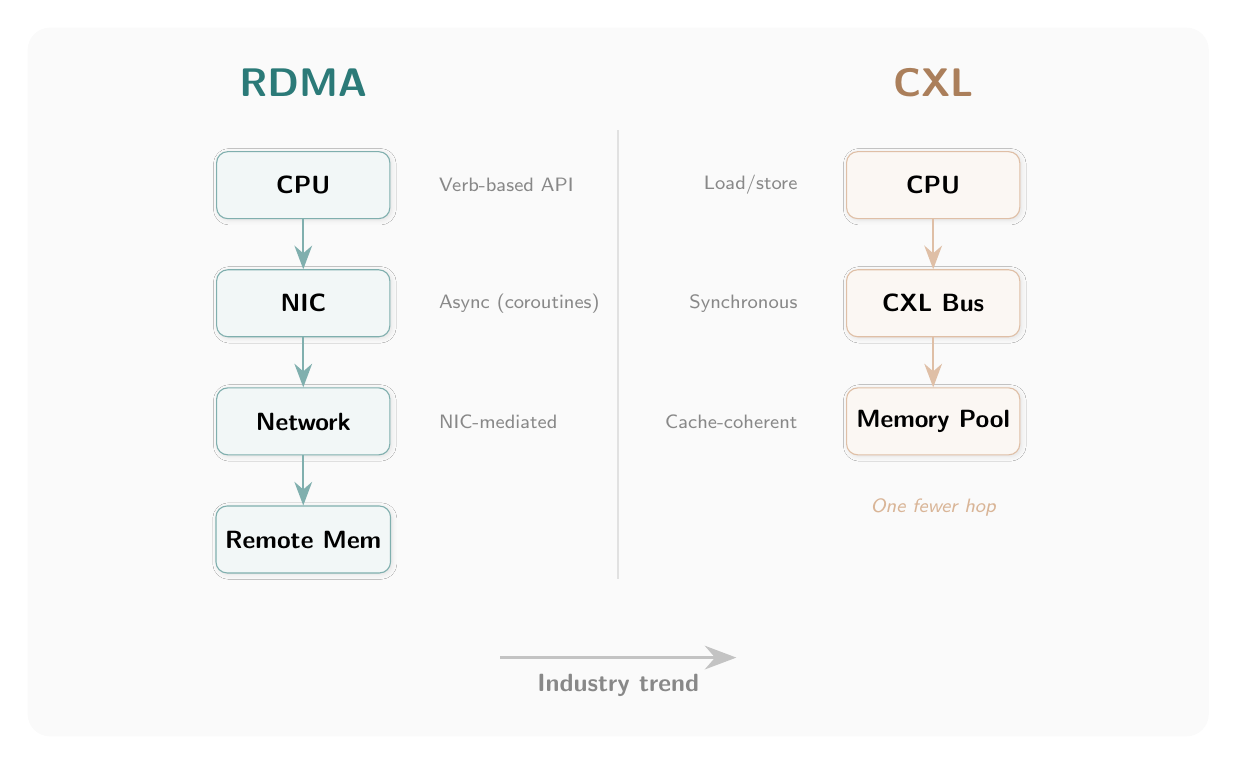
\begin{tikzpicture}[
  every node/.style={font=\sffamily},
  rbox/.style={draw=mTeal!60, fill=mTeal!6, rounded corners=4pt,
               minimum width=2.2cm, minimum height=0.85cm, font=\sffamily\small,
               blur shadow={shadow blur steps=4, shadow xshift=0.2mm,
               shadow yshift=-0.2mm, shadow opacity=10}},
  cbox/.style={draw=mBrown!60, fill=mBrown!8, rounded corners=4pt,
               minimum width=2.2cm, minimum height=0.85cm, font=\sffamily\small,
               blur shadow={shadow blur steps=4, shadow xshift=0.2mm,
               shadow yshift=-0.2mm, shadow opacity=10}},
  lbl/.style={font=\sffamily\scriptsize, mGray},
  >=Stealth,
]
  \fill[mBg, rounded corners=8pt] (-7.5,-4.5) rectangle (7.5,4.5);

  % Headers
  \node[font=\sffamily\Large\bfseries, mTeal] at (-4, 3.8) {RDMA};
  \node[font=\sffamily\Large\bfseries, mBrown!85!black] at (4, 3.8) {CXL};

  % Divider
  \draw[mGray!25, thick] (0,3.2) -- (0,-2.5);

  % RDMA path
  \node[rbox] (r1) at (-4, 2.5) {\textbf{CPU}};
  \node[rbox] (r2) at (-4, 1) {\textbf{NIC}};
  \node[rbox] (r3) at (-4,-0.5) {\textbf{Network}};
  \node[rbox] (r4) at (-4,-2) {\textbf{Remote Mem}};

  \draw[-{Stealth[length=3mm]}, thick, mTeal!60] (r1) -- (r2);
  \draw[-{Stealth[length=3mm]}, thick, mTeal!60] (r2) -- (r3);
  \draw[-{Stealth[length=3mm]}, thick, mTeal!60] (r3) -- (r4);

  \node[lbl, anchor=west] at (-2.4, 2.5) {Verb-based API};
  \node[lbl, anchor=west] at (-2.4, 1) {Async (coroutines)};
  \node[lbl, anchor=west] at (-2.4,-0.5) {NIC-mediated};

  % CXL path
  \node[cbox] (c1) at (4, 2.5) {\textbf{CPU}};
  \node[cbox] (c2) at (4, 1) {\textbf{CXL Bus}};
  \node[cbox] (c3) at (4,-0.5) {\textbf{Memory Pool}};

  \draw[-{Stealth[length=3mm]}, thick, mBrown!60] (c1) -- (c2);
  \draw[-{Stealth[length=3mm]}, thick, mBrown!60] (c2) -- (c3);

  \node[lbl, anchor=east] at (2.4, 2.5) {Load/store};
  \node[lbl, anchor=east] at (2.4, 1) {Synchronous};
  \node[lbl, anchor=east] at (2.4,-0.5) {Cache-coherent};

  % Fewer steps highlight
  \node[mBrown!70, font=\sffamily\scriptsize\itshape] at (4,-1.6) {One fewer hop};

  % Industry trend
  \draw[-{Stealth[length=4mm, width=3mm]}, very thick, mGray!50]
    (-1.5,-3.5) -- (1.5,-3.5)
    node[midway, below=2pt, font=\sffamily\small\bfseries, mGray] {Industry trend};
\end{tikzpicture}
\end{document}
